%this file is the second report
%a % comment anything after % until the end of the line

%minimum references to begin our article
\documentclass[12pt]{article}
\usepackage[english]{babel}
\usepackage[utf8]{inputenc}
\usepackage[T1]{fontenc}
\usepackage{graphicx}
\usepackage{fancyhdr}
\usepackage{hyperref}
\usepackage{float}
\usepackage{enumitem}
\usepackage{amsmath}
\usepackage[margin=1in]{geometry}
\usepackage{indentfirst}
\usepackage{titlesec}
\usepackage{verbatim}
\usepackage{url}
\newcommand{\sectionbreak}{\clearpage}

%\setlength{\parskip}{10pt plus 1pt minus 1pt} %Adds spacing between paragraphs 
\usepackage{parskip}
\setlength{\parindent}{15pt}

\pagestyle{fancy}
%\cfoot{Fast and furious game playing: Monte Carlo drift}
% the last extension makes it possible to add images

%presentation of the document
\title{Fast and Furious Game Playing: Monte Carlo Drift\smallbreak Planning report} %not sure about the name of this report
\author{Prateek \textsc{Bhatnagar}, Baptiste \textsc{Bignon}, \\
        Mikaïl \textsc{Demirdelen}, Gabriel \textsc{Prevosto}, \\
        Dan \textsc{Seeruttun-{}-Marie}, Benoît \textsc{Viguier} \\
        \\
        Supervisors: Nikolaos \textsc{Parlavantzas}, Christian \textsc{Raymond}}
\date{12/19/2014}
\setlength\parindent{15pt}
\begin{document}
\maketitle

\begin{figure}[!h] 
\centerline{\includegraphics[scale=0.50]{Pictures/arimaa}}
\end{figure}
\newpage

%to add a table of contents
\tableofcontents
\newpage


\section{Introduction}					\label{sec:introduction} 		
Our project is called Fast and furious game playing, MonteCarlo drift. Our purpose is to create an Artificial Intelligence able to compete against humans using the MonteCarlo Tree Research.
\newline
We will only focus on two players games. Furthermore, we want to avoid games already resolved. We will choose something not studied entirely. We want to work on some new application. That is why we are interested by Arimaa.
\newline
\newline
For our game, we will need a program and statistics to make a good Artificial Intelligence. Each move should be calculated using a reliable method.
MonteCarlo Tree Research is an algorithm able to take these optimal decisions. It has been used in the past for draughts, or chess. By exploring numerous possibilities, it will become possible to know what move is the better one.
We will parallelize this algorithm in order to use it in a multi-core machine, to improve his efficiency.
That MCTS algorithm is better than the classic Min-Max algorithm, that is why we will use it.
\newline
\newline
We will analyse parallelization methods, we will present it, and then we will choose the one adapted to our project.
Thanks to the results of these latest methods, we will be able to choose a state resulting of the current move. Then we will explore the tree and with the same methods as before, we will figure out what the opponent will most probably do. The way we will be exploring the tree will only depend on the parallelization method.
The first part of our project will be the analysis of latest thesis of technologies we will use, in order to choose the best one, and using it on the right environment, to improve his  efficiency.
In the next part, we will choose technologies we will need to achieve our goals, we will create a UML diagram to settle down our program.
\newline
\newline
Finally, in the last part, we will implement this program, and its documentation and test his executing on Grid5000, a cluster of multi-core machines.
What is interesting in this project is we will create an Artificial Intelligence using technologies and methods fully optimized. Then we will create a program that can lead to true improvements for current algorithms applied to this game.



\newpage

\section{Planning Methods}				\label{sec:PlanningMethods}
	\subsection{Presentation Methods}		\label{sec:PresentationMethods}		%\subsection{The Minimax algorithm}
% miss the blank space
The Minimax algorithm is a way of finding an optimal move in a two player game. In the search tree for a two player game, there are two kinds of nodes, nodes representing ones moves and nodes representing the opponent's moves.\cite{graphics_minimax}
\begin{figure}[H]
\centering
	\begin{minipage}[b]{0.45\linewidth}
		\centering
		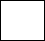
\includegraphics[height=1cm]{2_State_of_the_art/Arimaa_on_MCTS_Benoit/img/max.png}
		\caption{\label{fig:max}Nodes representing ones moves are generally drawn as squares, these are also called \emph{MAX} nodes.}
	\end{minipage}%
	\hspace*{1cm}
	\begin{minipage}[b]{0.45\linewidth}
		\centering
		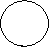
\includegraphics[height=1cm]{2_State_of_the_art/Arimaa_on_MCTS_Benoit/img/min.png}
		\caption{\label{fig:min}Nodes representing the opponent's moves are generally drawn as circles, these are also called \emph{MIN} nodes.}
	\end{minipage}%
\end{figure}

The goal of a \emph{MAX/MIN} node is to maximize/minimize the value of the subtree rooted at that node. To do this, a \emph{MAX/MIN} node chooses the child with the greatest/smallest value, and that becomes the value of the \emph{MAX/MIN} node.

Note that it's typical for two player games to have different branching factors at each node. The move one makes could have an impact on what moves are possible for the opponent. In this example, one is ignoring what the game is in order to focus on the algorithm.

\begin{figure}[H]
\centering
	\begin{minipage}[b]{0.45\linewidth}
		\centering
		\includegraphics[height=1.5cm]{2_State_of_the_art/Arimaa_on_MCTS_Benoit/img/Minimax2.png}
		\caption{\label{fig:Minimax2}At the start of the problem, Minimax checks the single present node.}
	\end{minipage}%
	\hspace*{1cm}
	\begin{minipage}[b]{0.45\linewidth}
		\centering
		\includegraphics[height=3cm]{2_State_of_the_art/Arimaa_on_MCTS_Benoit/img/Minimax3.png}
		\caption{\label{fig:Minimax3}It begins like a depth first search, generating the first child.}
	\end{minipage}%
\end{figure}

So far we've really seen no evaluation values. The way Minimax works is to go down a specified number of full moves (where one \emph{full move}' is actually a move by each player), then calculate the evaluation values for states at that depth. For this example, we're going to go down one full move, which is one more level.
\begin{figure}[H]
\centering
	\begin{minipage}[b]{0.45\linewidth}
		\centering
		\includegraphics[height=3cm]{2_State_of_the_art/Arimaa_on_MCTS_Benoit/img/Minimax4.png}
		\caption{\label{fig:Minimax4}we generate the values for those nodes.}
	\end{minipage}%
	\hspace*{1cm}
	\begin{minipage}[b]{0.45\linewidth}
		\centering
		\includegraphics[height=3cm]{2_State_of_the_art/Arimaa_on_MCTS_Benoit/img/Minimax5.png}
		\caption{\label{fig:Minimax5}It chooses the minimum of the two child node values, which is 3.}
	\end{minipage}%
\end{figure}

The max node at the top still has two other children nodes that we need to generate and search.

\begin{figure}[H]
\centering
	\begin{minipage}[b]{0.45\linewidth}
		\centering
		\includegraphics[height=3cm]{2_State_of_the_art/Arimaa_on_MCTS_Benoit/img/Minimax6.png}
		\caption{\label{fig:Minimax6}Since there is only one child, the min node must take it's value.}
		\end{minipage}%
	\hspace*{1cm}
	\begin{minipage}[b]{0.45\linewidth}
		\centering
		\includegraphics[height=3cm]{2_State_of_the_art/Arimaa_on_MCTS_Benoit/img/Minimax8.png}
		\caption{\label{fig:Minimax8}The third min node chooses the minimum of it's child node values, 1.}
	\end{minipage}%
\end{figure}

Finally we have all of the values of the children of the max node at the top level, so it chooses the maximum of them, 15, and we get the final solution. 

\begin{figure}[H]
\centering
	\begin{minipage}[b]{1\linewidth}
		\centering
		\includegraphics[height=3cm]{2_State_of_the_art/Arimaa_on_MCTS_Benoit/img/Minimax9.png}
		\caption{\label{fig:Minimax9}Final tree.}
	\end{minipage}%
\end{figure}

What this tells us is that we should take the move that leads to the middle min node, since it'll lead to the best possible state for us one full move down the road.

\subsection{The \ensuremath{\alpha\beta} pruning} %pruning = elaguage en anglais
The \ensuremath{\alpha\beta} method is a heuristic that decrease the number of leaf that will be explored by the Minimax algorithm. That way, the size of the tree will be smaller, the algorithm will be able to dive further and the time spend on more interesting subtree is greater.\\
If the leaf's position is less interesting than its parents, the algorithm won't explore anyfurther.

\subsection{Monte Carlo Tree Search Algorithm}
\subsubsection{Introduction}
Monte Carlo Tree Search (MCTS) is an algorithm used for taking decisions in Artificial Intelligence (AI) problems such as solving games or decision making in project managment. It is based on making a big number of random simulations in order to get trustfull datas. To make such simulations, the program play the moves randomly for each players. Once it reach a conclusion (win or loss), the program compute the statistics to get the odds of winning.
\subsubsection{How does it works ?}
The Algorithm create a tree with all possible solution with a small depth.
Then it start to run random simulations starting from the leaves in order to test the odds of the outcome.
Once we got enough the results (usually we are using time based simulations) we feed back the results and make the decision depending on the odds of each subsequent leaves.
\subsubsection{Example}
\label{sec:example}
\begin{figure}[H]
\centering
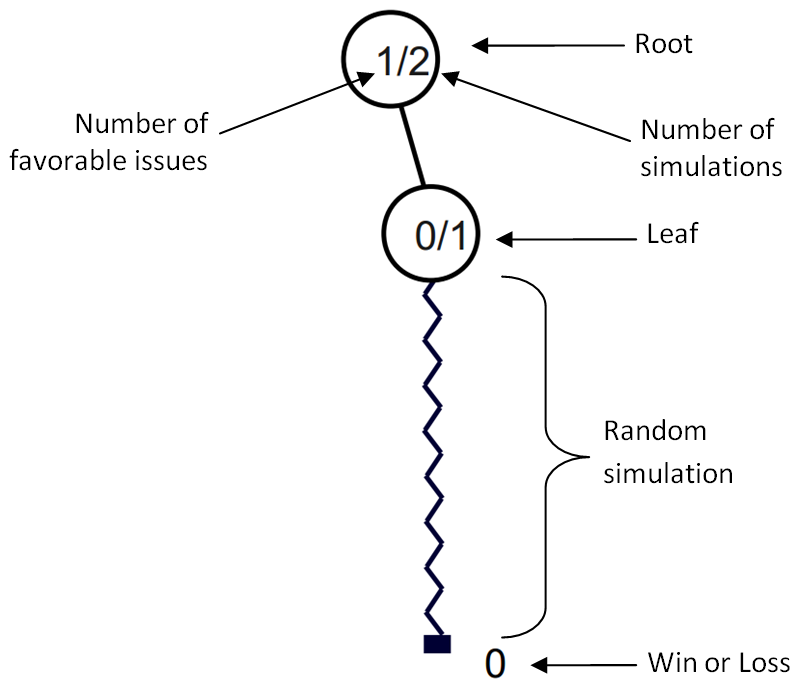
\includegraphics[height=5cm]{1_Presentation/1.2_Algorithm_MCTS_Benoit/img/schema.png}
\caption{\label{fig:schema}Legend of the following figures.}
\end{figure}

\begin{figure}[H]
\centering
	\begin{minipage}[b]{0.45\linewidth}
		\centering
		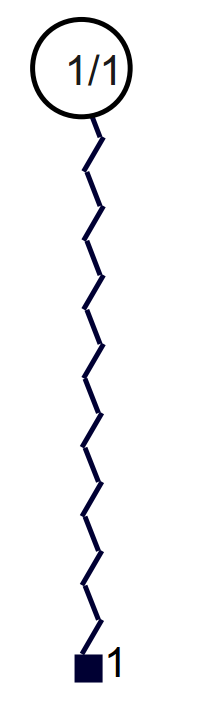
\includegraphics[height=4cm]{1_Presentation/1.2_Algorithm_MCTS_Benoit/img/1.png}
		\caption{\label{fig:1}Run a first simulation from the root, get a favorable issue (will be considered as a \textit{win}).}
	\end{minipage}%
	\hspace*{1cm}
	\begin{minipage}[b]{0.45\linewidth}
		\centering
		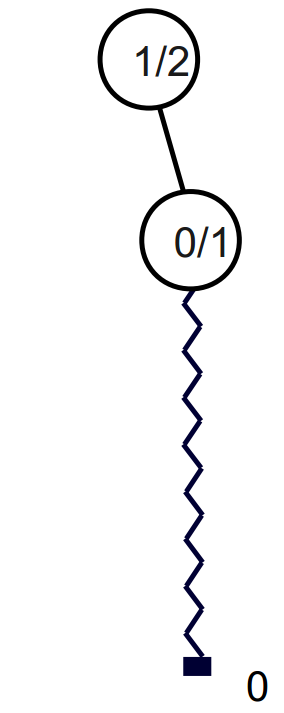
\includegraphics[height=4cm]{1_Presentation/1.2_Algorithm_MCTS_Benoit/img/2.png}
		\caption{\label{fig:2}Create a first leaf at depth 1 and run the simulation, get an unfavorable issue (considered as a \textit{loss}).}
	\end{minipage}%
\end{figure}

\begin{figure}[H]
\centering
	\begin{minipage}[b]{0.3\linewidth}
		\centering
		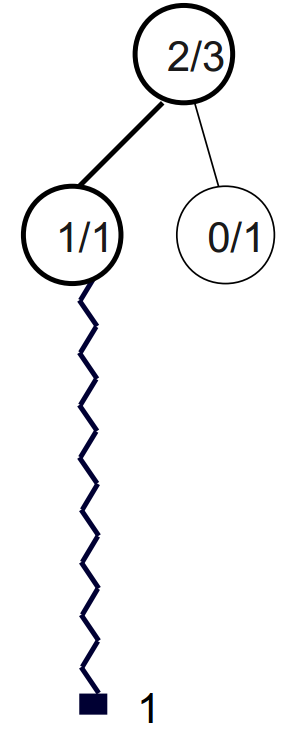
\includegraphics[height=4cm]{1_Presentation/1.2_Algorithm_MCTS_Benoit/img/3.png}
		\caption{\label{fig:3}Create a second leaf at depth 1 and run the simulation (\textit{win}).}
	\end{minipage}%
	\hspace*{1cm}
	\begin{minipage}[b]{0.3\linewidth}
		\centering
		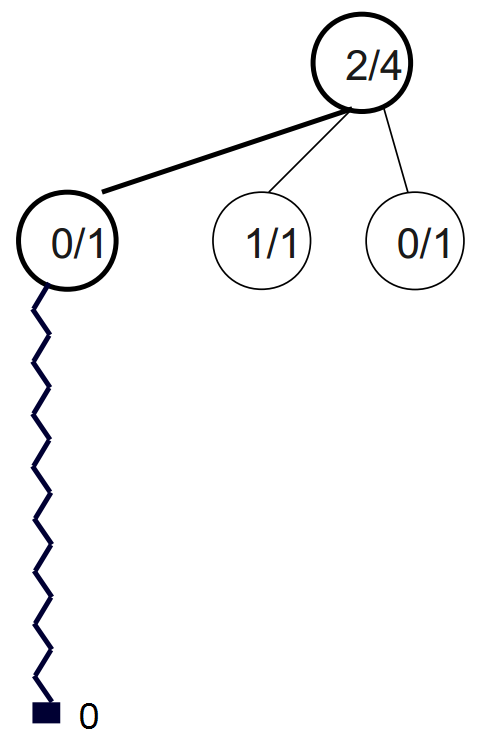
\includegraphics[height=4cm]{1_Presentation/1.2_Algorithm_MCTS_Benoit/img/4.png}
		\caption{\label{fig:4}Create a third leaf at depth 1 and run the simulation (\textit{loss}).}
	\end{minipage}%
	\hspace*{1cm}
	\begin{minipage}[b]{0.3\linewidth}
		\centering
		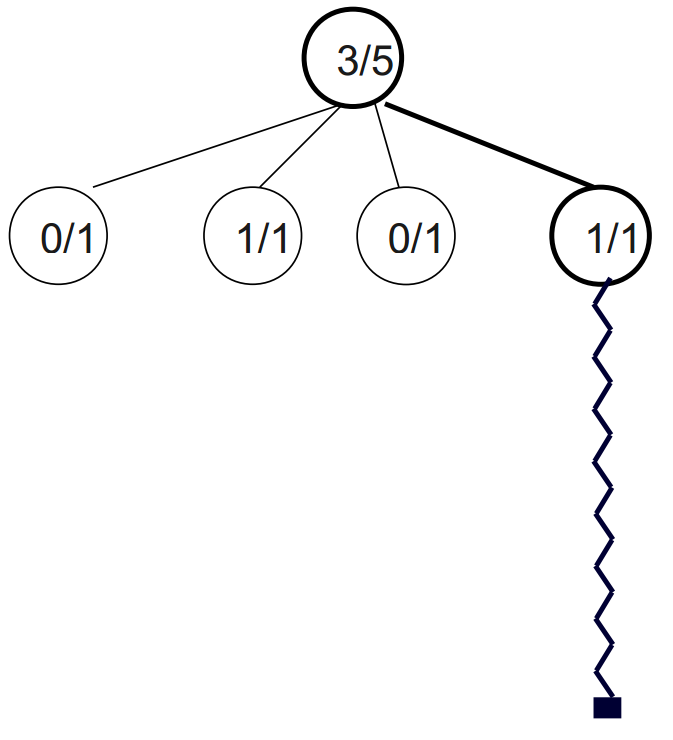
\includegraphics[height=4cm]{1_Presentation/1.2_Algorithm_MCTS_Benoit/img/5.png}
		\caption{\label{fig:5}Create a fourth leaf at depth 1 and run the simulation (\textit{win}).}
	\end{minipage}%
\end{figure}

Right now the odds of winning are 3/5. Now that we tested all the possible outcomes at depth 1, we will expend the tree on the favorable leaves (here the second and fourth).

\begin{figure}[H]
\centering
	\begin{minipage}[b]{0.45\linewidth}
		\centering
		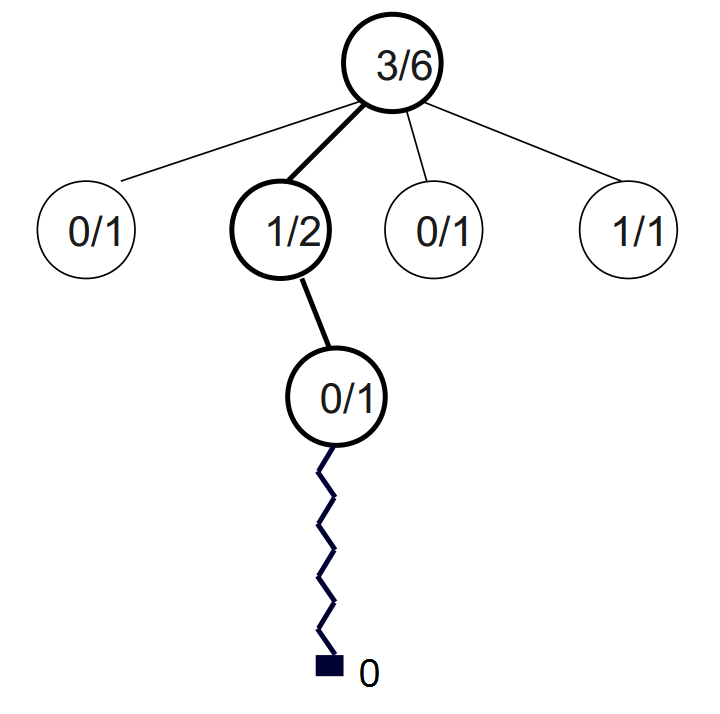
\includegraphics[height=4cm]{1_Presentation/1.2_Algorithm_MCTS_Benoit/img/6.png}
		\caption{\label{fig:6}Create a leaf at depth 2 with parent the 2nd leaf at depth 1 and run the simulation (\textit{loss}), update the odds value of the node and making it less interesting than the fourth node. Therefore the algorithm will now work on the fourth node.}
	\end{minipage}%
	\hspace*{1cm}
	\begin{minipage}[b]{0.45\linewidth}
		\centering
		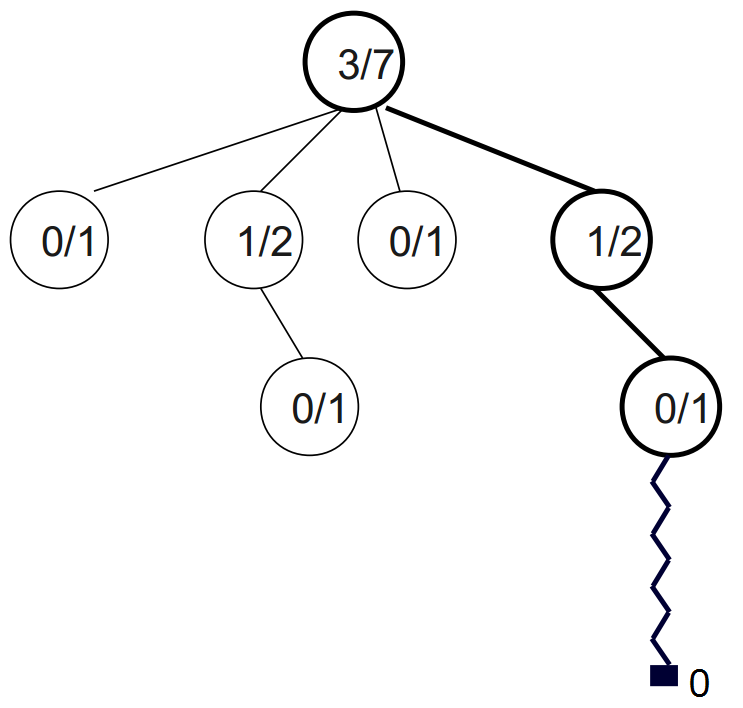
\includegraphics[height=4cm]{1_Presentation/1.2_Algorithm_MCTS_Benoit/img/7.png}
		\caption{\label{fig:7}Create a leaf at depth 2 with parent the fourth leaf at depth 1 and run the simulation (\textit{loss}), update the odds value of the node and making it as interesting as the second node. The algorithm will now work on the second node.}
	\end{minipage}%
\end{figure}
\begin{figure}[H]
\centering
	\begin{minipage}[b]{0.45\linewidth}
		\centering
		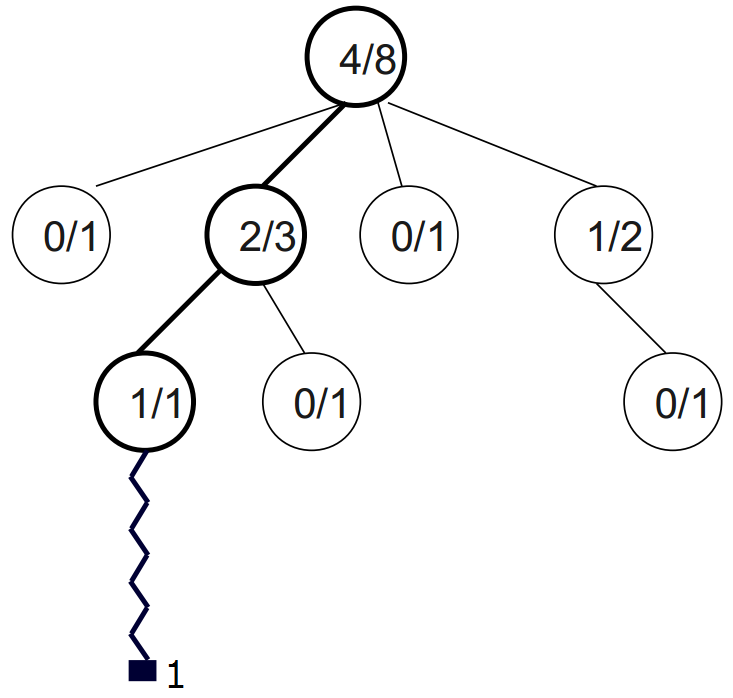
\includegraphics[height=4cm]{1_Presentation/1.2_Algorithm_MCTS_Benoit/img/8.png}
		\caption{\label{fig:8}Create a second leaf at depth 2 with parent the second leaf at depth 1 and run simulation (\textit{win}), update the odds value and continue to develop this leaf.}
	\end{minipage}%
	\hspace*{1cm}
	\begin{minipage}[b]{0.45\linewidth}
		\centering
		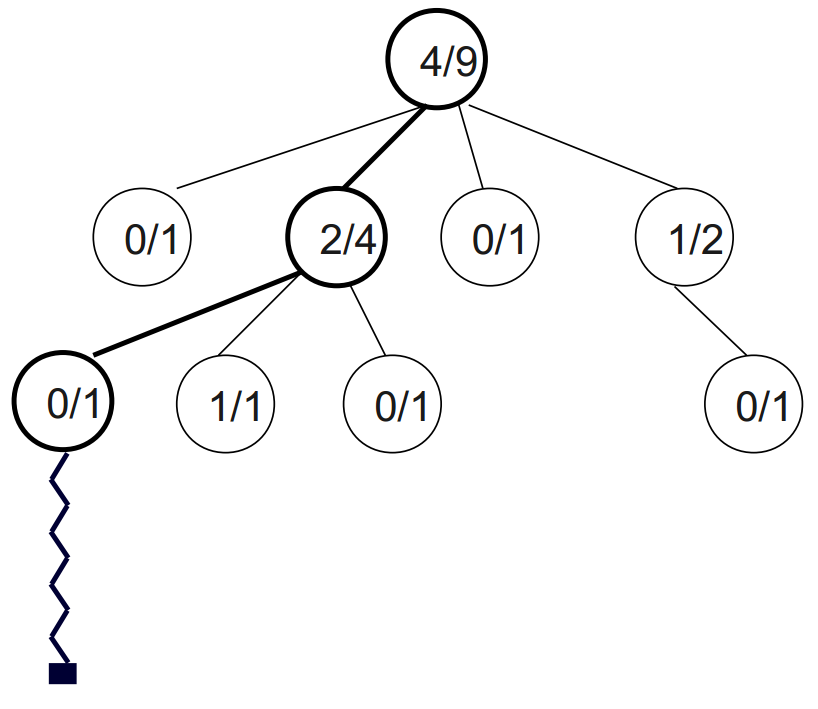
\includegraphics[height=4cm]{1_Presentation/1.2_Algorithm_MCTS_Benoit/img/9.png}
		\caption{\label{fig:9}Create a third leaf at depth 2 with parent the second leaf at depth 1 and run simulation (\textit{loss}), update the odds value and switch to the fourth leaf.\null\\}
	\end{minipage}%
\end{figure}

Continue the Algorithm until a decent about of simulation are run and/or the time limit is .
\begin{figure}[H]
\centering
	\begin{minipage}[b]{0.33\linewidth}
	\centering
		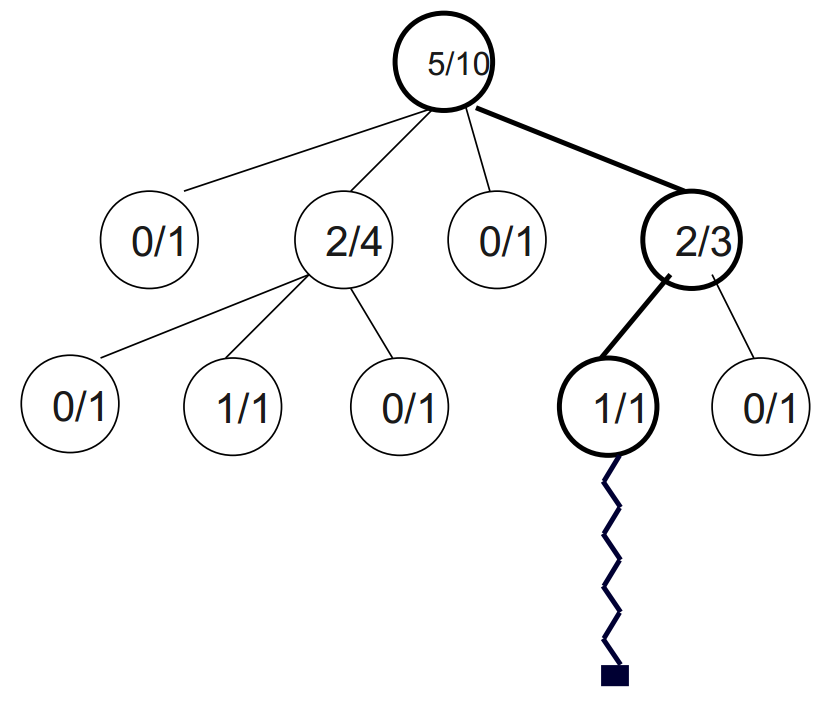
\includegraphics[height=4cm]{1_Presentation/1.2_Algorithm_MCTS_Benoit/img/10.png}
	\end{minipage}%
	\begin{minipage}[b]{0.33\linewidth}
	\centering
		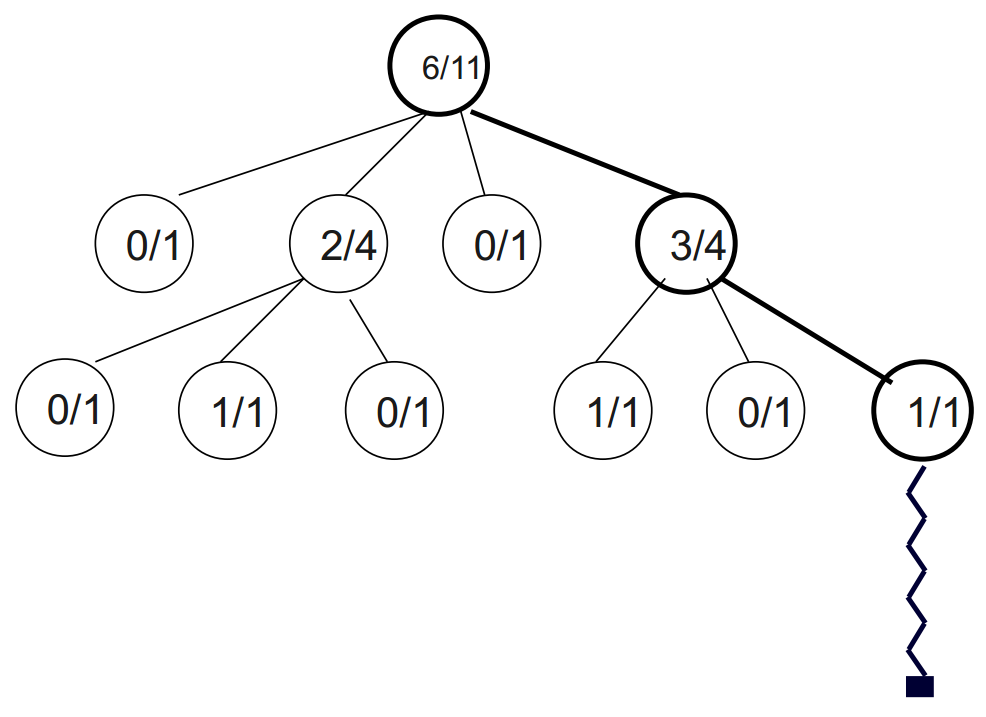
\includegraphics[height=4cm]{1_Presentation/1.2_Algorithm_MCTS_Benoit/img/11.png}
	\end{minipage}%
	\begin{minipage}[b]{0.33\linewidth}
	\centering
		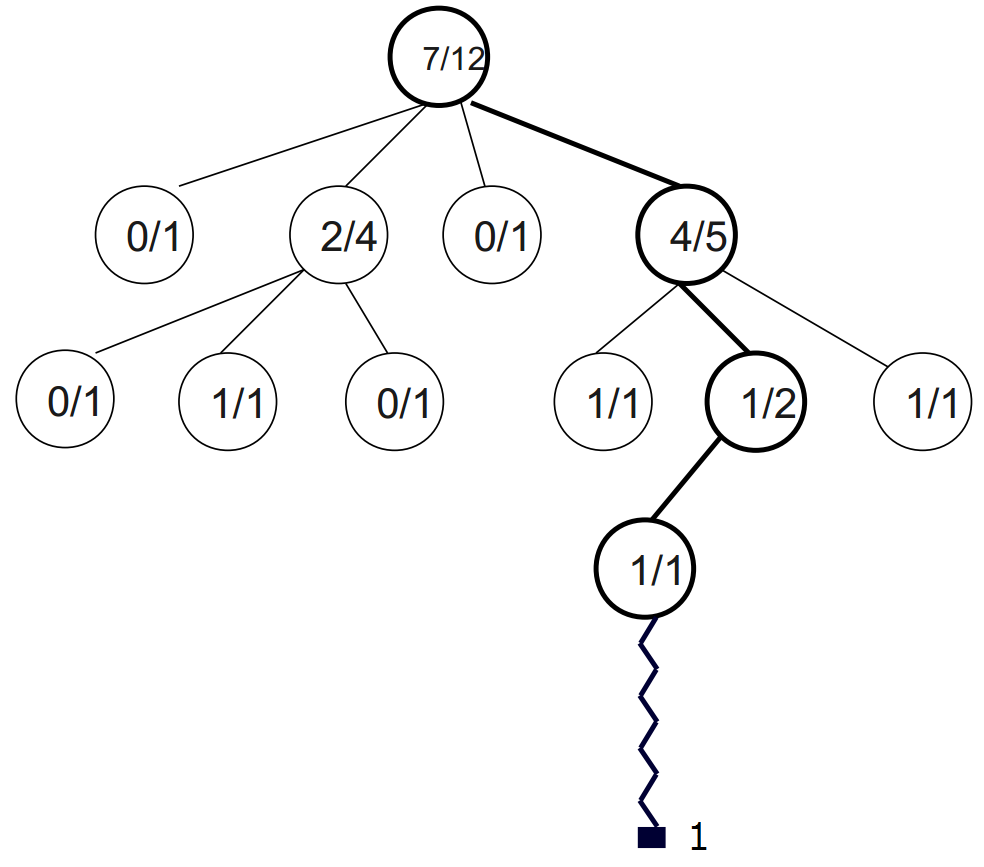
\includegraphics[height=4cm]{1_Presentation/1.2_Algorithm_MCTS_Benoit/img/12.png}
	\end{minipage}%
\end{figure}

Make a decision : here we chose the fourth leaf.\\
\newpage
\subsubsection{How to select the leaves to develop ?}
In the previous exemple, we chose to not expend leaves without winrates. But depending on the results of the simulations, wins can vary greatly. Therefore we will run more simulations on each leaf before chosing the ones to develop. For practical purpose we will select the leaves to expend that has the highest value of the cost function UCT (Upper Confidence Bound 1 applied to Trees).\\
\bigskip
\begin{minipage}[b]{1\linewidth}
\centering
\begin{equation*}
f = \frac{w_i}{n_i} + c\sqrt{\frac{\ln t}{n_i}}
\end{equation*}
\medskip
\textit{UCT function}\cite{formula_UCT}

\end{minipage}%
\bigskip
\begin{itemize}
  \item \ensuremath{w_i} : number of wins after the ith node
  \item \ensuremath{n_i} : number of simulations after the ith node
  \item \ensuremath{c}   : exploration parameter – theoretically equal to \ensuremath{\sqrt{2}} but in practice chosen empirically
  \item \ensuremath{t}   : total number of simulations in a given tree node, equal to the sum of all \ensuremath{n_i}
\end{itemize}
\medskip
The more a leaf is developed, the less it's cost is worth it. This way we can be sure that a leaf with low winrate isn't completely forgotten.\\

\subsubsection{Why using the Monte Carlo Tree Search ?}
 The advantage of MCTS with it's basic form is that you don't need to implement functions to improve the researches. Based on its random simulations, it will determine by itself which are the good options and which aren't.\\ The more you run simulations, the more accurate the results will be.

\subsubsection{How much power do we need ?}
The more the game has possible moves, the more power it require to solve. In order to get decisions, it needs to go deeper in the tree and to search enough leaves. If the time or number of simulations is not sufficient, the algorithm might miss some important branches and fail to give plausible results. Therefore in order to get decent results, using high-end computer is mandatory, it allows us to get access to multi-threading technology in order to parallelize the simulations.
	\subsection{Environment}			\label{sec:environment}			\subsubsection{Human Resources}

Our project group is composed of six students, half of which will be abroad next semester.
That implies that most of the development phase will be carried out by a team of three people, with the help of the supervisors.
We also hope to get some advice from Mr Garcia, a researcher from INSA who knows a lot about Artificial Intelligence.

\subsubsection{Other resources}

The algorithm is due to exploit parallelization in order to give more accurate results. We will first test it on the machines from INSA's Computer Science department;
then, if we have the time and the authorization required, we will run it on \emph{Grid'5000}, a set of clusters of multi-core machines.

\subsubsection{Exterior knowledge}

The Artificial Intelligence (\emph{AI}) will implement the \emph{Monte Carlo Tree Search} (\emph{MCTS}) algorithm, that has been used in the past for board games.
The AI will be parallelized using the \emph{Root parallelization} strategy, one of the main strategies used with the MCTS algorithm.

\subsubsection{Technologies used}

A few technologies will be used for this project:
\begin{itemize}
	\item The project will be coded using the C++ language
	\item The application providing a user interface uses SFML 1.6
	\item Either MPI, OpenMP and OpenACC or an implemntation of the actor model (such as \emph{CAF}) will be used for parallelization
\end{itemize}

\subsubsection{Important dates}

For this project, a number of set deadlines exist:
\begin{itemize}
	\item A conception report is due by the 12$^{th}$  of February
	\item A HTML documentation is due by the 25$^{th}$ of March
	\item The final report  is due by the 26$^{th}$ of May
	\item A demonstration of the AI will take place on the 26$^{th}$ of May
	\item The application is to be finished and sent by the 28$^{th}$ of May
	\item A presentation of the project will take place on the 28$^{th}$ of May
\end{itemize}

In order to give us more time to work on the project, some time has been freed on our schedule, from May the 18$^{th}$ to May the 28$^{th}$.
On the other hand, the exams that take place on the weeks of January the 12$^{th}$ and May the 11$^{th}$ have been considered as time off the project. 
Outside of these time periods, the workload for each member of the team has been set to 4 hours a week, in order to increase our flexibility.
\newpage

\section{Task Planning}					\label{sec:generalArchitecture} 		
	\subsection{Tasks list for Gant diagram}	\label{sec:Gantt}			\subsubsection{Tasks gathered in modules}

To understand better how the tasks are organized, tasks have been classified in modules, representing the main aspects of our project. Each task will be checked, and tested just after, according to the Agile method.

\begin{itemize}
  \item The first module is the GUI application. It contains a Graphical Interface for our game, but as well the rules to play, and a recorder of rules. 
This application will make it possible for an human to play against another human.
  \item The second module is the MCTS algorithm. It is the heart of our project. This algorithm will be used to compute a set of all moves possible ordered in a tree. First, it will be implemented on \textit{Tic-Tac-Toe}, then on \textit{Connect4} and finally on \textit{Arimaa}. 

With this module, it will be possible to play against the AI.
There will be as well some improvements to do as the use of Boost library, a better memory management, and making statistics.
  \item The module Converter is a converter of data to make communicate the MCTS part and the GUI part.
  \item The Parallelization module represents the management of our environment. Our algorithm will be tested using different computer powers, with CPU and GPU parallelization. It will be tested on our computers, on the computers of our INSA computer science department. Finally, if the time permits us, we will test it on the researchers' network \textit{Grid'5000}. 

This module will increase the performances of our algorithm, giving it calculus power.
  \item The last module is the Documentation. It will take a lot of our time, writing 2 reports, preparing 2 oral presentations, conceiving an HTML page and a CD of the application.
\end{itemize}
All these tasks form part of the Gantt diagram.

\subsubsection{Gantt diagram}
\includepdf[
	landscape = true,
    pages = 1,
    turn = false,
    angle=180
	]
{C:/Users/ishamael/Documents/GitHub/Arimaa/Docs/Reports/Report_3/TasksPlanning/GanttDiagram/Gantt_v1.pdf}
	\subsection{Risks analysis}			\label{sec:Risks}			There will always be problems or delays that come up. The best way to deal with them is to think about what could go wrong in the Project rather than waiting to get into deep water. The five kinds of risks are the following :
\begin{enumerate}
	\item technical
	\item Ressources
	\item Organisation
	\item Payments
	\item Suppliers/Purchases
\end{enumerate}
Our main risk factors is the point number 1 : technical. We are not dependant to anything like purchases, ressources or organisation as we are a small group of workers and we barely need anything but our computer.\\
To get into further details, here is a list of what might possibly become cumbersome :
\begin{itemize}
	\item getting used to the technology we will use (CAF, OpenMPI, OpenAcc, OpenMP, Boost Library...)
	\item booking the use of Grid5000, we don't know how long is the waiting list in order to be able to borrow it.
	\item Interoperability problems : most of us works on Windows Operating Systems. However Grid5000 runs on Linux, for this reason we will test our algorithm on a smaller scale. The computer science departement at INSA will be our first testing facility in order to make our cluster implemtation works.
\end{itemize}
Some other problems might come up later and we will try to deal with them as soon as possible to get the least delay as we possibly could.~\\

\newpage


\section{Conclusion}					\label{sec:conclusion}	%		
The main focus area of this report is planning. Various planning methods have been decided such as Agile development methodology and Planning Poker method.
Using Agile Development Methodology, the incremental  development of the project will take place. Planning Poker method  which is the estimation technique of Agile Methodology is used to estimate the time requirement for the development of the project. The dates have been estimated with respect to the development of various models of our project.A serious attempt is made analyse the risks  in order to take preventive measures to avoid various risks and problems. 

\newpage

%uncomment to add bibliography
%\bibliography{bibliography}
%\bibliographystyle{plain}

\end{document}
